\documentclass[journal]{IEEEtran}
\usepackage{amsmath,amsfonts,amssymb,amsthm}
\usepackage{algorithmic}
\usepackage{algorithm}
\usepackage{array}
\usepackage{booktabs}
\usepackage{multirow}
\usepackage[caption=false,font=normalsize,labelfont=sf,textfont=sf]{subfig}
\usepackage{textcomp}
\usepackage{stfloats}
\usepackage{url}
\usepackage{verbatim}
\usepackage{graphicx}
\usepackage{cite}
\usepackage{xcolor}
\hyphenation{op-tical net-works semi-conduc-tor IEEE-Xplore}

\newtheorem{definition}{Definition}
\newtheorem{proposition}{Proposition}
\newtheorem{lemma}{Lemma}

\begin{document}

\title{SELENE: Selective Empathy LoRA with Factor Gates\\
for English--Korean Affective Transfer}

\author{Jaehong~Kim,
Seohyeon~Yoo,
and Jaehyuk~Cho%
\thanks{J. Kim, S. Yoo, and J. Cho are with the Department of Software Engineering,
Jeonbuk National University, Jeonju, Republic of Korea
(corresponding author: J. Cho; e-mail: chojh@jbnu.ac.kr).}%
\thanks{Manuscript received XXX XX, 2026; revised XXX XX, 2026.
Working draft targeting \textit{IEEE Transactions on Affective Computing}.
Backbone: \texttt{Qwen/Qwen3.5-9B}.}}

\markboth{IEEE Transactions on Affective Computing,~Vol.~XX, No.~X, XXX~2026}%
{Kim \MakeLowercase{\textit{et al.}}: SELENE for EN--KO Empathetic Transfer}

\IEEEpubid{0000--0000/00\$00.00~\copyright~2026 IEEE}

\maketitle

\begin{abstract}
Large language models that perform well on English empathetic dialogue often fail to transfer that competence to Korean, where empathy is shaped by relational stance, honorifics, and high-context support strategies.
We propose \textbf{SELENE} (\textbf{S}elective \textbf{E}mpathy \textbf{L}oRA with \textbf{EN}--KO factor gat\textbf{E}s): a parameter-efficient EN$\rightarrow$KO affective transfer system on a frozen \texttt{Qwen/Qwen3.5-9B} backbone.
SELENE (i)~pretrains an English empathy LoRA with an affect head on EmpatheticDialogues, (ii)~assigns factor-wise share/relearn/suppress gates from EN--KO divergence and frozen probes, and (iii)~adapts a Korean LoRA with multitask affect, strategy, and relation supervision on AI~Hub dialogues.
Unlike language$\times$task adapter merging alone, SELENE gates theoretically motivated empathy factors (Affect / Cognition / Strategy / Relation).
We evaluate two directions: Direction~I Korean A/S/R accuracy versus non-selective baselines, and Direction~II return-to-English performance after KO adaptation (gain versus forgetting), with KoED held out for cultural evaluation.
Illustrative comparisons suggest that Affect/Cognition are largely shareable while Strategy/Relation require relearning---motivating selective gates over blind EN adapter copy.
\end{abstract}

\begin{IEEEkeywords}
Affective computing, empathetic dialogue, cross-lingual transfer, LoRA, cultural adaptation, Korean NLP, support strategies.
\end{IEEEkeywords}

\section{Introduction}
\IEEEPARstart{E}{mpathetic} response generation is a core affective computing problem that couples emotion understanding with socially appropriate generation~\cite{rashkin2019empathetic,liu2021esc,sharma2020empathy}.
Open-domain empathy benchmarks such as EmpatheticDialogues (ED)~\cite{rashkin2019empathetic} and emotional-support corpora such as ESC~\cite{liu2021esc} have driven rapid progress in English, and large language models (LLMs) further improve fluency on affective tasks~\cite{amin2024chatgpt,sabour2024emobench}.
Yet multilingual competence does not imply multicultural empathy~\cite{lee2025koed,zhou2024culture,ahuja2023mega}: models that score well in English frequently violate Korean relational norms, over-empathize, or select support strategies that are pragmatically odd in honorific, high-context settings~\cite{lee2025koed,matsumoto2008culture}.

A common remedy is full fine-tuning on Korean dialogues.
This is compute-heavy and risks catastrophic forgetting of English affective skills~\cite{kirkpatrick2017overcoming,wang2022lfmlf}.
Parameter-efficient fine-tuning (PEFT), especially LoRA~\cite{hu2022lora} and modular adapters~\cite{houlsby2019adapters,pfeiffer2020madx}, reduces cost and keeps the backbone frozen.
However, typical EN$\rightarrow$KO transfer still treats empathy as a \emph{monolithic} skill: either copy an English adapter blindly, train Korean from scratch, or merge language$\times$task adapters without asking which \emph{empathy factors} should be shared versus relearned~\cite{zhao2025adamerge,borchert2025flare}.

Psychological and dialogue research argues that empathy is multidimensional~\cite{davis1983empathy}: affective sharing, perspective-taking, helping strategies, and culturally regulated display rules are separable.
ESC further shows that support \emph{strategy}---not emotion mirroring alone---drives perceived helpfulness~\cite{liu2021esc,sharma2020empathy}.
KoED demonstrates a measurable cultural empathy gap between ED and culturally reconstructed Korean dialogues~\cite{lee2025koed}.
Together, these observations motivate \emph{factor-selective} transfer rather than uniform adapter reuse.

This paper asks: can we transfer English empathy to Korean selectively at the level of theoretically motivated affective factors, while keeping the backbone frozen and preserving return-to-English performance?

Our contributions are:
\begin{enumerate}
\item A theory-aligned A/C/S/R factor schema for empathetic dialogue (Affect, Cognition, Strategy, Relation), anchored in empathy theory, ESC strategies, and Korean relational norms~\cite{davis1983empathy,liu2021esc,matsumoto2008culture,lee2025koed}.
\item \textbf{SELENE}, implementing Factor-LoRA SELECT: English LoRA pretraining, divergence/probe gating (share/relearn/suppress), and gated Korean multitask LoRA adaptation on frozen \texttt{Qwen/Qwen3.5-9B}.
\item A dual evaluation protocol---Direction~I (EN$\rightarrow$KO affective accuracy) and Direction~II (return-to-EN after KO)---plus stage-wise ablations that isolate EN pretraining, gates, and multitask heads.
\item A unified EN--KO data pipeline over EmpatheticDialogues, KoED, KorEmpatheticDialogues, and AI~Hub under one JSONL schema, with factor-wise EN--KO comparison figures that justify selective gates.
\end{enumerate}
\IEEEpubidadjcol

\section{Related Work}

\subsection{Empathetic and Emotional Support Dialogue}
EmpatheticDialogues remains the standard open-domain empathy benchmark for emotion-grounded response generation~\cite{rashkin2019empathetic}.
Subsequent systems emphasize mixture-of-experts emotion routing~\cite{lin2019moel}, emotion mimicking~\cite{majumder2020mime}, and commonsense-aware empathy~\cite{sabour2022cem}.
Emotional Support Conversation (ESC) shows that staged helping strategies (exploration$\rightarrow$comforting$\rightarrow$action) improve support effectiveness beyond affect mirroring~\cite{liu2021esc}.
Computational empathy metrics for support text further highlight explorations, interpretations, and emotional reactions as complementary axes~\cite{sharma2020empathy}.
EmoBench evaluates multi-faceted emotional intelligence in LLMs~\cite{sabour2024emobench}, and broad TAFFC evaluations report uneven LLM behavior across affective tasks~\cite{amin2024chatgpt}.
Our Strategy~(S) axis follows ESC and is operationalized with AI~Hub labels (advice / encourage / comfort / agree), while Affect~(A) uses emotion labels from ED and AI~Hub.

\subsection{Cultural Empathy and Multilingual Evaluation}
KoED is our problem mother paper~\cite{lee2025koed}: multilingual LLMs underperform on culturally reconstructed Korean dialogues relative to ED (emotion Acc $36.84\!\rightarrow\!32.69$ on shared emotions), and cultural appropriateness favors Korean-aligned models.
This aligns with broader evidence that LLMs exhibit Western-centric cultural defaults even when prompted in other languages~\cite{zhou2024culture}, and that multilingual benchmarks must separate linguistic fluency from cultural competence~\cite{ahuja2023mega,ponti2020xcopa}.
Cross-cultural psychology motivates Relation~(R) through display rules and emotion regulation under social context~\cite{matsumoto2008culture}.
SELENE does not replace culturally aligned pretraining; instead it provides a PEFT mechanism to \emph{selectively} adapt English empathy factors toward Korean A/S/R supervision while freezing a shared backbone.

\subsection{Parameter-Efficient Cross-Lingual Transfer}
Adapter modules~\cite{houlsby2019adapters} and LoRA~\cite{hu2022lora} enable low-rank task adaptation without updating all backbone weights.
MAD-X separates language and task adapters for modular cross-lingual transfer~\cite{pfeiffer2020madx}.
AdaMergeX merges task/language LoRAs with adaptive arithmetic and reports large gains over MAD-X-style baselines~\cite{zhao2025adamerge}.
FLARE fuses EN/target representations inside LoRA bottlenecks and improves target-language accuracy over plain LoRA~\cite{borchert2025flare}.
Strong multilingual encoders such as XLM-R underpin much of this transfer stack~\cite{conneau2020xlmr}.
On the forgetting side, classical continual-learning results warn that sequential adaptation can erase prior skills~\cite{kirkpatrick2017overcoming}, and LF-MLF shows that reducing source-side forgetting improves retained multilingual transfer~\cite{wang2022lfmlf}---motivating our Direction~II return-to-EN protocol.
These methods operate at language$\times$task granularity; SELENE instead gates empathy factors A/S/R with share/relearn/suppress decisions.

\section{Problem Formulation}
Let $x$ be a dialogue context and $y$ an empathetic listener response.
We do \emph{not} claim a unique latent decomposition of empathy.
Instead we give operational definitions, testable propositions, and analytic consequences of the gate map that jointly justify factor-selective transfer.

\subsection{Definitions}
\begin{definition}[Theory-aligned factors]
\label{def:factors}
Let $\mathcal{K}=\{A,C,S,R\}$.
For each factor $k\in\mathcal{K}$, an observable label space $\mathcal{Y}_k$ is fixed a priori by theory and corpus annotation (Table~\ref{tab:factors}):
$A$~=~emotion, $C$~=~situation/appraisal proxy, $S$~=~support strategy, $R$~=~relation type~\cite{davis1983empathy,rashkin2019empathetic,liu2021esc,matsumoto2008culture,lee2025koed}.
When $y_C$ is unavailable as a discrete label, $C$ is treated as a \emph{proxy} factor and excluded from gated decisions unless otherwise stated.
\end{definition}

\begin{definition}[Factor representation and head]
\label{def:repr}
Let $h_\theta(x)\in\mathbb{R}^{d}$ be the pooled hidden state of a frozen backbone (with optional EN LoRA).
Define $z_k(x):=P_k h_\theta(x)$ with projection $P_k$ (identity in the current prototype; factor subspaces / LoRA banks in the full system).
A factor head $f_k$ predicts $\hat{y}_k=f_k(z_k(x))$.
\end{definition}

\begin{definition}[Transfer score and gate map]
\label{def:score}
On Korean labeled pairs $\{(x_i^{\mathrm{KO}},y_{k,i})\}$, the transfer score is
\begin{equation}
\label{eq:sk}
s_k
=
\mathrm{Acc}\!\big(f_k^{\mathrm{probe}};\, h_\theta(x^{\mathrm{KO}}),\, y_k^{\mathrm{KO}}\big)
\in[0,1],
\end{equation}
optionally mixed with an EN--KO alignment term.
Fix thresholds $1\ge\tau_{\mathrm{share}}>\tau_{\mathrm{suppress}}\ge 0$.
The three intervals
$[0,\tau_{\mathrm{suppress}}]$,
$(\tau_{\mathrm{suppress}},\tau_{\mathrm{share}})$,
$[\tau_{\mathrm{share}},1]$
form a partition of $[0,1]$, so there is a unique map
\begin{equation}
\label{eq:gates}
g_k=\Gamma(s_k)
=
\begin{cases}
\mathrm{share}, & s_k \ge \tau_{\mathrm{share}},\\
\mathrm{suppress}, & s_k \le \tau_{\mathrm{suppress}},\\
\mathrm{relearn}, & \text{otherwise,}
\end{cases}
\end{equation}
sending each score to one gate.
Equip gates with the total order
$\mathrm{suppress}\prec\mathrm{relearn}\prec\mathrm{share}$
(``more sharing'' is larger).
\end{definition}

\begin{definition}[Gate-conditioned LoRA init]
\label{def:init}
Let $M_{\mathrm{EN}}$ be the Stage~1 English LoRA and $\mathrm{Rand}$ a matched-rank random init.
The init operator $\mathcal{I}$ maps a gate to a KO LoRA seed:
\begin{equation}
\label{eq:init}
\mathcal{I}(g)
=
\begin{cases}
M_{\mathrm{EN}}, & g=\mathrm{share},\\
\mathrm{Rand}, & g=\mathrm{relearn},\\
\rho\,M_{\mathrm{EN}}, & g=\mathrm{suppress},
\end{cases}
\end{equation}
with scale $\rho\in[0,1)$ (soft attenuation of EN directions).
For factor set $\mathcal{K}$, Stage~3 seeds are
$M_{\mathrm{KO}}^{(0)}=\{\mathcal{I}(\Gamma(s_k))\}_{k\in\mathcal{K}}$.
\end{definition}

We write $z=(z_A,z_C,z_S,z_R)$ as shorthand for Definition~\ref{def:repr}.
English pretraining yields transferable components of $z_A$ (and proxy $z_C$); Korean requires culture-specific realization especially for $z_S$ and $z_R$~\cite{lee2025koed}.
The learning objective maximizes Korean A/S/R accuracy (Direction~I) subject to limited degradation of English emotion recognition after KO adaptation (Direction~II).

\subsection{Propositions and Gate Lemmas}
\begin{proposition}[Separability]
\label{prop:sep}
For each $k\in\{A,S,R\}$, a linear probe $f_k$ on frozen $h_\theta(x^{\mathrm{KO}})$ satisfies
$\mathrm{Acc}_k \ge \mathrm{chance}_k+\delta$ for a pre-registered margin $\delta>0$
(e.g., $\delta{=}0.1$), under a held-out KO split.
\end{proposition}

\begin{proposition}[Partial non-redundancy]
\label{prop:indep}
For $k\neq k'$, cross-factor probe accuracy $\mathrm{Acc}(f_k\!\to\! y_{k'})$ is significantly lower than $\mathrm{Acc}(f_k\!\to\! y_k)$,
and/or Cram\'{e}r's $V(y_k,y_{k'})$ remains below a redundancy ceiling $V_0$.
\end{proposition}

\begin{proposition}[Transfer ordering]
\label{prop:order}
Under an EN Stage~1 encoder, transfer scores obey
$s_A \ge \tau_{\mathrm{share}}$ and $s_S,s_R < \tau_{\mathrm{share}}$
(equivalently $s_A,s_C \gg s_S,s_R$ when $C$ is scored),
supporting share for affect(/cognition) and relearn for strategy/relation.
\end{proposition}

\begin{proposition}[Gated intervention]
\label{prop:intervene}
With matched backbone, rank, and budget,
$\mathrm{DirI}(\mathrm{SELECT})>\mathrm{DirI}(\mathrm{Blind})$
and
$|\Delta_{\mathrm{DirII}}(\mathrm{SELECT})|\le|\Delta_{\mathrm{DirII}}(\mathrm{Blind})|$,
where Blind uses $\Gamma\equiv\mathrm{share}$.
\end{proposition}

\begin{lemma}[Monotone gate and local stability]
\label{lem:gate}
Under Definition~\ref{def:score}, $\Gamma$ is (i)~monotone nondecreasing w.r.t.\ $\prec$, and (ii)~locally constant away from thresholds.
Precisely: if $s\le s'$, then $\Gamma(s)\preceq\Gamma(s')$.
Moreover, if
$\mathrm{dist}\!\big(s,\{\tau_{\mathrm{suppress}},\tau_{\mathrm{share}}\}\big)\ge\varepsilon>0$,
then every $s'$ with $|s'-s|<\varepsilon$ satisfies $\Gamma(s')=\Gamma(s)$.
\end{lemma}
\begin{proof}
Monotonicity follows because crossing a threshold can only move a score into a weakly higher gate region under $\prec$; within a region $\Gamma$ is constant.
For stability, the open $\varepsilon$-ball about $s$ cannot reach either threshold, hence lies in the same partition cell as $s$, so $\Gamma$ is unchanged.
\end{proof}

\begin{lemma}[Induced init is score-determined]
\label{lem:init}
The Stage~3 seed map $s\mapsto\mathcal{I}(\Gamma(s))$ is uniquely determined by Definitions~\ref{def:score}--\ref{def:init}.
If $\mathrm{dist}(s_k,\{\tau_{\mathrm{suppress}},\tau_{\mathrm{share}}\})\ge\varepsilon$ and $|\hat{s}_k-s_k|<\varepsilon$, then
$\mathcal{I}(\Gamma(\hat{s}_k))=\mathcal{I}(\Gamma(s_k))$:
bootstrap/probe noise that stays off the threshold boundaries does not flip the KO LoRA seed.
\end{lemma}
\begin{proof}
Immediate from uniqueness of $\Gamma$ on the partition and Lemma~\ref{lem:gate}(ii), composed with the deterministic map $\mathcal{I}$ in~\eqref{eq:init}.
\end{proof}

\subsection{Validation Protocol}
Propositions~\ref{prop:sep}--\ref{prop:intervene} are \emph{empirical claims}, not existence theorems.
We verify them by: (i)~KO held-out probes for~\eqref{eq:sk}; (ii)~cross-factor Acc / Cram\'{e}r's $V$; (iii)~bootstrap tests of the ordering in Proposition~\ref{prop:order}; (iv)~gated vs.\ blind / all-relearn interventions for Proposition~\ref{prop:intervene}; (v)~seed/fold stability of $\{g_k\}$ and of $M_{\mathrm{KO}}^{(0)}$ under Lemma~\ref{lem:init}.
Lemmas~\ref{lem:gate}--\ref{lem:init} are analytic consequences of the definitions; they do \emph{not} prove that A/C/S/R is the unique empathy factorization.
Only after~(iii)--(iv) hold do we apply $\{g_k\}$ via $\mathcal{I}\circ\Gamma$ in Stage~3.

\section{Method: SELENE (Factor-LoRA SELECT)}
SELENE is the system name; Factor-LoRA SELECT is the three-stage algorithm.
Unless noted, we freeze \texttt{Qwen/Qwen3.5-9B}---size-matched to KoED open peers ($\sim$7--8B)~\cite{lee2025koed}---and train only LoRA adapters plus lightweight A/S/R heads.
Fig.~\ref{fig:overview} shows the pipeline; Fig.~\ref{fig:directions} shows the two evaluation directions; Fig.~\ref{fig:gates} summarizes the gate rule.

\begin{figure}[!t]
\centering
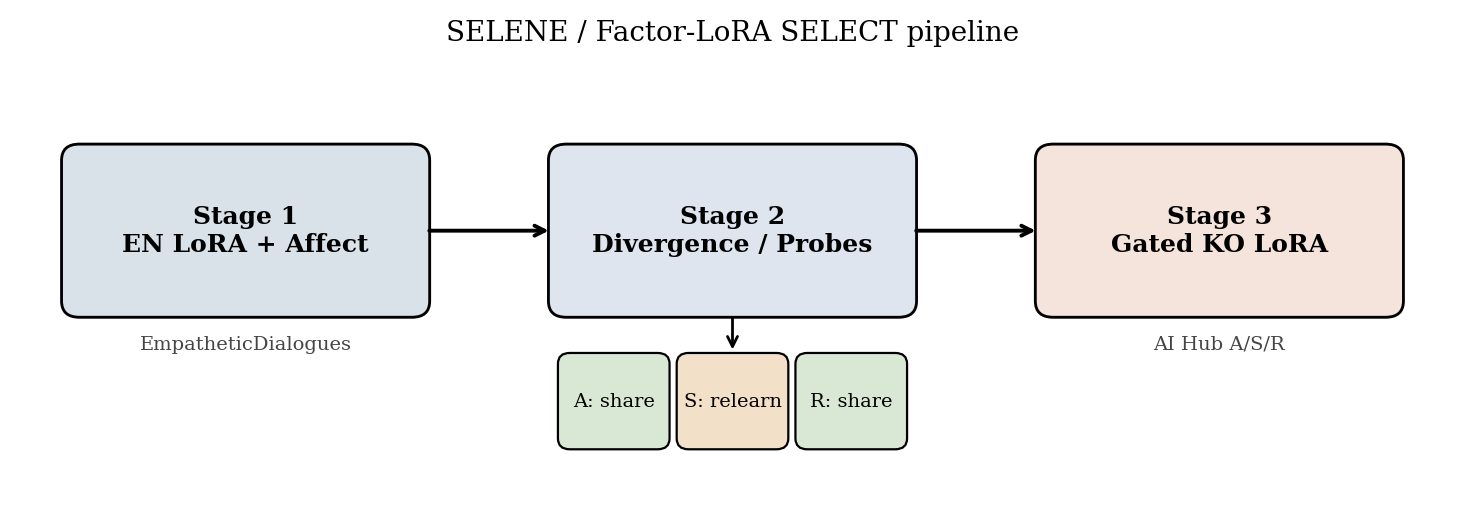
\includegraphics[width=\columnwidth]{figures/fig_overview.png}
\caption{SELENE overview: English empathy LoRA, factor-wise gates, then gated Korean multitask adaptation.}
\label{fig:overview}
\end{figure}

\begin{figure}[!t]
\centering
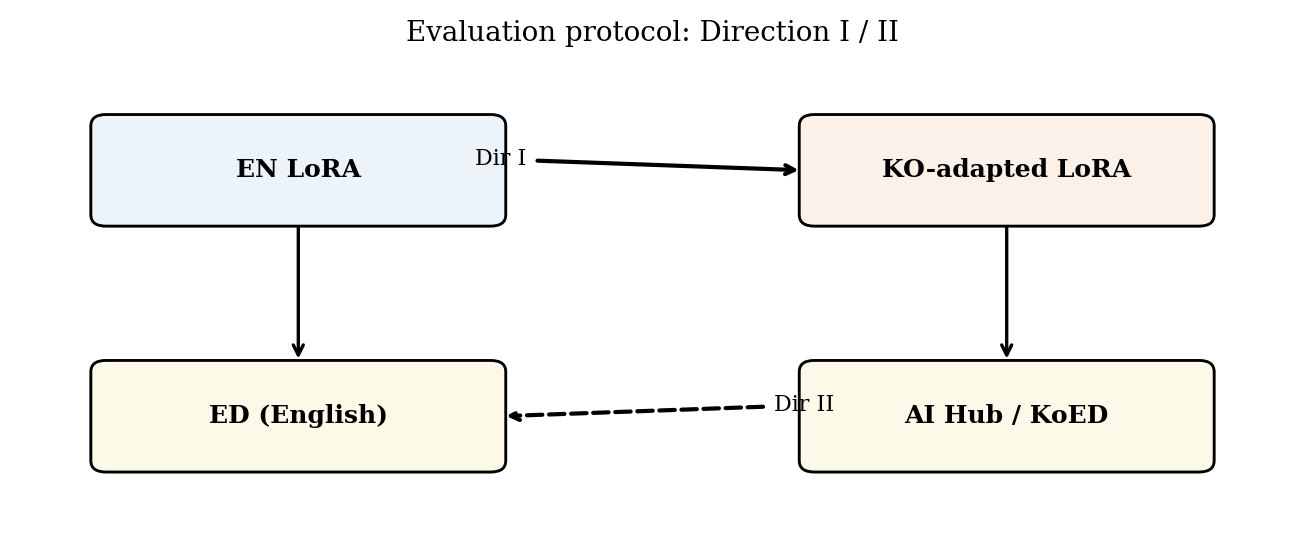
\includegraphics[width=\columnwidth]{figures/fig_directions.png}
\caption{Evaluation protocol. Direction~I measures Korean A/S/R accuracy; Direction~II returns to English ED after KO adaptation.}
\label{fig:directions}
\end{figure}

\begin{figure}[!t]
\centering
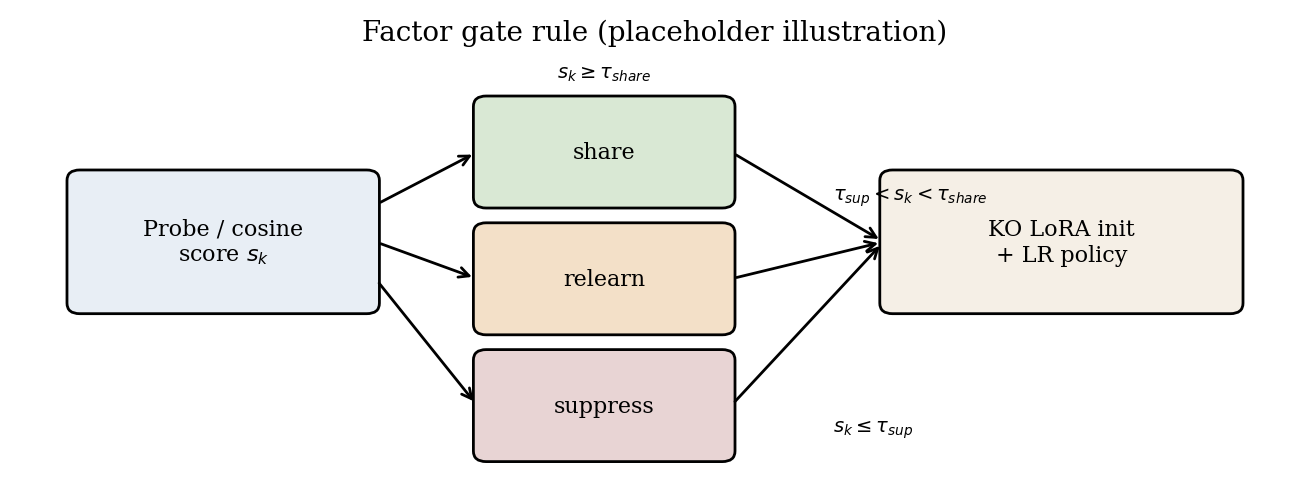
\includegraphics[width=\columnwidth]{figures/fig_gates.png}
\caption{Factor gate rule mapping probe/similarity scores to share / relearn / suppress (illustrative).}
\label{fig:gates}
\end{figure}

\subsection{Theory-Based Factor Definition}
Table~\ref{tab:factors} lists pre-defined factors and literature anchors.
Divergence analysis is used to \emph{validate} these factors, not to invent them post hoc from clusters.
Davis separates empathic concern (A) from perspective-taking (C)~\cite{davis1983empathy}; Rashkin operationalizes emotion + situation in ED~\cite{rashkin2019empathetic}; ESC supplies strategy supervision (S)~\cite{liu2021esc}; Matsumoto and KoED motivate relational/cultural display constraints (R)~\cite{matsumoto2008culture,lee2025koed}.

\begin{table}[!t]
\caption{Theory-Aligned Empathy Factors}
\label{tab:factors}
\centering
\resizebox{\columnwidth}{!}{%
\begin{tabular}{@{}lll@{}}
\toprule
Factor & Theory & Operational label \\
\midrule
A Affect & Empathic concern~\cite{davis1983empathy} & Emotion (ED / AI~Hub) \\
C Cognition & Perspective-taking~\cite{davis1983empathy} & Situation text (proxy) \\
S Strategy & ESC helping skills~\cite{liu2021esc} & Advice / encourage / comfort / agree \\
R Relation & Display rules + KO norms~\cite{matsumoto2008culture,lee2025koed} & AI~Hub relation types \\
\bottomrule
\end{tabular}%
}
\end{table}

\subsection{Stage 1: English Empathy LoRA}
On EmpatheticDialogues we train a causal LM with LoRA and an affect classification head on pooled prompt states:
\begin{equation}
\label{eq:en_loss}
\mathcal{L}_{\mathrm{EN}}=\mathcal{L}_{\mathrm{LM}}+\lambda_A\mathcal{L}_{\mathrm{CE}}(A).
\end{equation}
This yields a reusable English empathy adapter $M_{\mathrm{EN}}$ while leaving $\theta$ intact, consistent with PEFT practice~\cite{hu2022lora}.

\subsection{Stage 2: Divergence / Probe Gates}
Stage~2 instantiates Definitions~\ref{def:score}--\ref{def:init}: with the frozen Stage-1 encoder we (i)~fit KO linear probes for A/S/R to obtain $s_k$ in~\eqref{eq:sk}, (ii)~optionally measure EN--KO / KoED alignment~\cite{lee2025koed}, and (iii)~apply $\Gamma$ in~\eqref{eq:gates} (Lemmas~\ref{lem:gate}--\ref{lem:init}).
When English lacks explicit S/R supervision, we prefer \textbf{relearn} unless probe evidence is strong.
Fig.~\ref{fig:factor_enko} and Table~\ref{tab:factor_enko} summarize the intended EN--KO pattern corresponding to Proposition~\ref{prop:order}: Affect/Cognition tend to align (share), while Strategy/Relation diverge and require relearning.

\begin{figure}[!t]
\centering
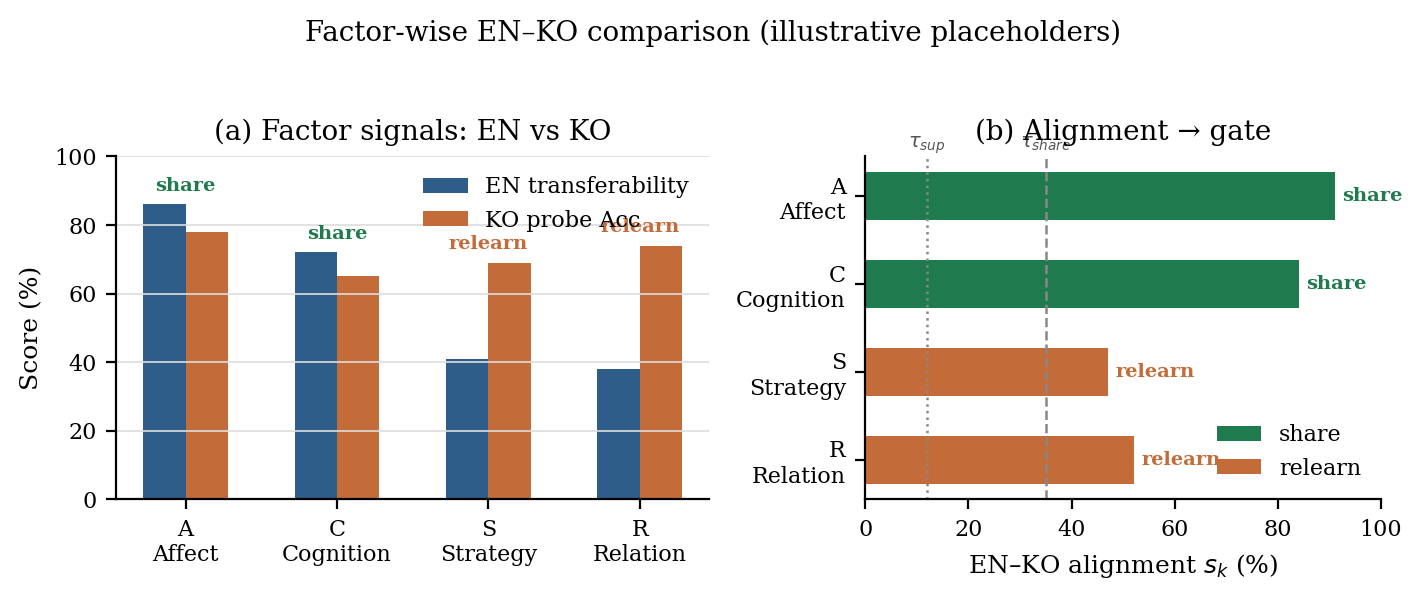
\includegraphics[width=\columnwidth]{figures/fig_factor_enko.png}
\caption{Factor-wise EN--KO comparison (illustrative placeholders).
(a)~EN transferability vs.\ KO probe Acc for A/C/S/R.
(b)~EN--KO alignment $s_k$ mapped to share/relearn gates.}
\label{fig:factor_enko}
\end{figure}

\begin{table}[!t]
\caption{Factor-wise EN--KO Pattern (illustrative; drives Stage~2 gates)}
\label{tab:factor_enko}
\centering
\resizebox{\columnwidth}{!}{%
\begin{tabular}{@{}lcccc@{}}
\toprule
Factor & EN signal & KO probe & Align $s_k$ & Gate \\
\midrule
A Affect & high & high & $0.91$ & share \\
C Cognition & mid--high & mid & $0.84$ & share \\
S Strategy & low & high & $0.47$ & relearn \\
R Relation & low & high & $0.52$ & relearn \\
\bottomrule
\end{tabular}%
}
\end{table}

\subsection{Stage 3: Gated Korean Adaptation}
On AI~Hub dialogues we set $M_{\mathrm{KO}}^{(0)}=\mathcal{I}(\Gamma(s_k))$ per factor (Definition~\ref{def:init}):
share copies $M_{\mathrm{EN}}$ (smaller LR to refine), relearn draws $\mathrm{Rand}$, and suppress applies $\rho M_{\mathrm{EN}}$.
We then train multitask objectives
\begin{equation}
\label{eq:ko_loss}
\mathcal{L}_{\mathrm{KO}}=\mathcal{L}_{\mathrm{LM}}+\lambda_A\mathcal{L}_A+\lambda_S\mathcal{L}_S+\lambda_R\mathcal{L}_R,
\end{equation}
so Korean adaptation is supervised not only for fluency but for A/S/R analysis heads, following the multi-axis empathy view in ESC and support-text evaluation~\cite{liu2021esc,sharma2020empathy}.
A composer weight $\alpha$ mixes EN$\oplus$KO adapters for Direction~II, preserving plug-in modularity~\cite{pfeiffer2020madx,zhao2025adamerge}.

\begin{algorithm}[t]
\caption{SELENE / Factor-LoRA SELECT}
\label{alg:select}
\begin{algorithmic}
\STATE Freeze backbone \texttt{Qwen/Qwen3.5-9B}
\STATE Stage~1: train EN LoRA + affect head on ED
\STATE Stage~2: encode EN/KO; assign gates $g_k$
\STATE \hspace{0.3cm} $g_k\in\{\mathrm{share},\mathrm{relearn},\mathrm{suppress}\}$
\STATE Stage~3: init KO LoRA from gates; train A/S/R
\STATE \textbf{return} EN LoRA, KO LoRA, $\{g_k\}$
\end{algorithmic}
\end{algorithm}

\section{Experimental Setup}

\subsection{Datasets and Backbone}
Table~\ref{tab:data} summarizes corpora.
AI~Hub provides full A/S/R labels; ED provides A/C; KoED is held out for cultural evaluation (not training), following~\cite{lee2025koed}.
KorEmpatheticDialogues serves as a translate-train control.
All main comparisons freeze \texttt{Qwen/Qwen3.5-9B} and match LoRA rank across systems; training curves in Fig.~\ref{fig:train} illustrate Stage~1/3 optimization dynamics.

\begin{table}[!t]
\caption{Dataset Statistics}
\label{tab:data}
\centering
\resizebox{\columnwidth}{!}{%
\begin{tabular}{@{}lcc@{}}
\toprule
Corpus & Role & Split size \\
\midrule
EmpatheticDialogues & EN Stage~1 / Dir~II & 17{,}844 / 2{,}763 / 2{,}542 \\
AI~Hub Empathetic Dial. & KO Stage~3 / Dir~I & 25{,}456 / 3{,}182 \\
KoED & Cultural eval (held out) & 1{,}360 (test) \\
KorEmpatheticDialogues & Translate-train baseline & 19{,}531 / 2{,}769 / 2{,}547 \\
\bottomrule
\end{tabular}%
}
\end{table}

\subsection{Literature Anchor (Mother Paper)}
Following KoED's controlled ED$\leftrightarrow$KoED comparison~\cite{lee2025koed}, Table~\ref{tab:koed_anchor} reprints their reported emotion-recognition averages.
This anchors Direction~I: even strong multilingual models drop on culturally adapted Korean empathy, so ``untouched multilingual'' is an insufficient upper bound.

\begin{table}[!t]
\caption{KoED Emotion Recognition Acc (\%). Reprinted averages from~\cite{lee2025koed} (not our runs).}
\label{tab:koed_anchor}
\centering
\setlength{\tabcolsep}{3.5pt}
\begin{tabular}{@{}lcccc@{}}
\toprule
& \multicolumn{2}{c}{ED (English)} & \multicolumn{2}{c}{KoED (Korean)} \\
\cmidrule(lr){2-3}\cmidrule(lr){4-5}
Model & w/o $j$/$h$ & w/ $j$/$h$ & w/o $j$/$h$ & w/ $j$/$h$ \\
\midrule
Llama-3.1-8B & 34.53 & 30.74 & 32.19 & 28.53 \\
Mistral-7B & 39.38 & 36.40 & 33.52 & 31.10 \\
Qwen2-7B & 32.73 & 30.74 & 25.70 & 22.57 \\
EXAONE-7.8B & 31.41 & 29.12 & 30.31 & 26.18 \\
Claude-3.5 & 46.17 & 42.94 & 41.72 & 38.31 \\
\midrule
\textbf{Average} & \textbf{36.84} & \textbf{33.99} & \textbf{32.69} & \textbf{29.34} \\
\bottomrule
\end{tabular}
\end{table}

\subsection{Systems}
Table~\ref{tab:systems} lists systems in a KoED-style checklist.
Baselines span no-transfer (Untouched KO), zero-shot EN (EN-only), non-selective PEFT (Blind share), translation supervision, and strong modular XLT peers (MAD-X / AdaMergeX / FLARE)~\cite{pfeiffer2020madx,zhao2025adamerge,borchert2025flare}.

\begin{table}[!t]
\caption{Systems Compared (Direction I/II)}
\label{tab:systems}
\centering
\resizebox{\columnwidth}{!}{%
\begin{tabular}{@{}llcc@{}}
\toprule
System & EN$\rightarrow$KO policy & Dir~I & Dir~II \\
\midrule
Untouched KO & KO LoRA from scratch (no EN init) & \checkmark & \checkmark \\
EN-only & Stage~1 EN LoRA on KO (no KO train) & \checkmark & --- \\
Blind share & Copy EN LoRA; no factor gates & \checkmark & \checkmark \\
Translate-train & KorED supervision & \checkmark & --- \\
MAD-X & Language + task adapters~\cite{pfeiffer2020madx} & \checkmark & --- \\
AdaMergeX & Adaptive adapter merge~\cite{zhao2025adamerge} & \checkmark & --- \\
FLARE & EN/target LoRA fusion~\cite{borchert2025flare} & \checkmark & --- \\
\midrule
\textbf{SELENE (ours)} & Factor gates share/relearn/suppress & \checkmark & \checkmark \\
\quad + compose $\alpha$ & EN$\oplus$KO mix on return-to-EN & --- & \checkmark \\
\bottomrule
\end{tabular}%
}
\end{table}

\subsection{Direction I --- Korean Affective Accuracy}
\textbf{Question:} Does selective transfer improve Korean A/S/R over non-selective baselines?
\textbf{Metrics:} Affect~(A), Strategy~(S), Relation~(R) Acc on AI~Hub valid; optional KoED CA (5-point) as in~\cite{lee2025koed,sharma2020empathy}.
Table~\ref{tab:dir_i} and Fig.~\ref{fig:dir_i} follow KoED's model$\times$metric layout.
\emph{Numbers are illustrative placeholders} pending full Qwen runs; best values in \textbf{bold}.
Under this placeholder regime, SELENE leads on Avg Acc and CA, with the largest relative lift on Strategy---consistent with ESC's claim that strategy is the fragile transfer dimension~\cite{liu2021esc}.

\begin{table*}[!t]
\caption{Direction I: Performance Comparison on Korean Empathetic Analysis (illustrative placeholders).
Primary metrics are A/S/R Acc (\%) on AI~Hub valid; KoED CA is 5-point.}
\label{tab:dir_i}
\centering
\begin{tabular}{@{}lccccc@{}}
\toprule
& \multicolumn{4}{c}{AI~Hub (Korean)} & KoED \\
\cmidrule(lr){2-5}\cmidrule(lr){6-6}
System & A Acc$\uparrow$ & S Acc$\uparrow$ & R Acc$\uparrow$ & Avg$\uparrow$ & CA$\uparrow$ \\
\midrule
Untouched KO & 52.1 & 48.5 & 44.0 & 48.2 & 2.94 \\
EN-only & 41.3 & 36.2 & 30.5 & 36.0 & 2.61 \\
Blind share & 55.4 & 54.0 & 46.8 & 52.1 & 3.12 \\
Translate-train & 53.0 & 50.1 & 45.2 & 49.4 & 3.05 \\
MAD-X & 56.2 & 55.5 & 48.1 & 53.3 & 3.18 \\
AdaMergeX & 57.8 & 56.9 & 49.0 & 54.6 & 3.27 \\
FLARE & 58.1 & 57.2 & 49.6 & 55.0 & 3.31 \\
\midrule
\textbf{SELENE (ours)} & \textbf{61.4} & \textbf{63.8} & \textbf{54.7} & \textbf{60.0} & \textbf{3.55} \\
\bottomrule
\end{tabular}
\end{table*}

\begin{figure*}[!t]
\centering
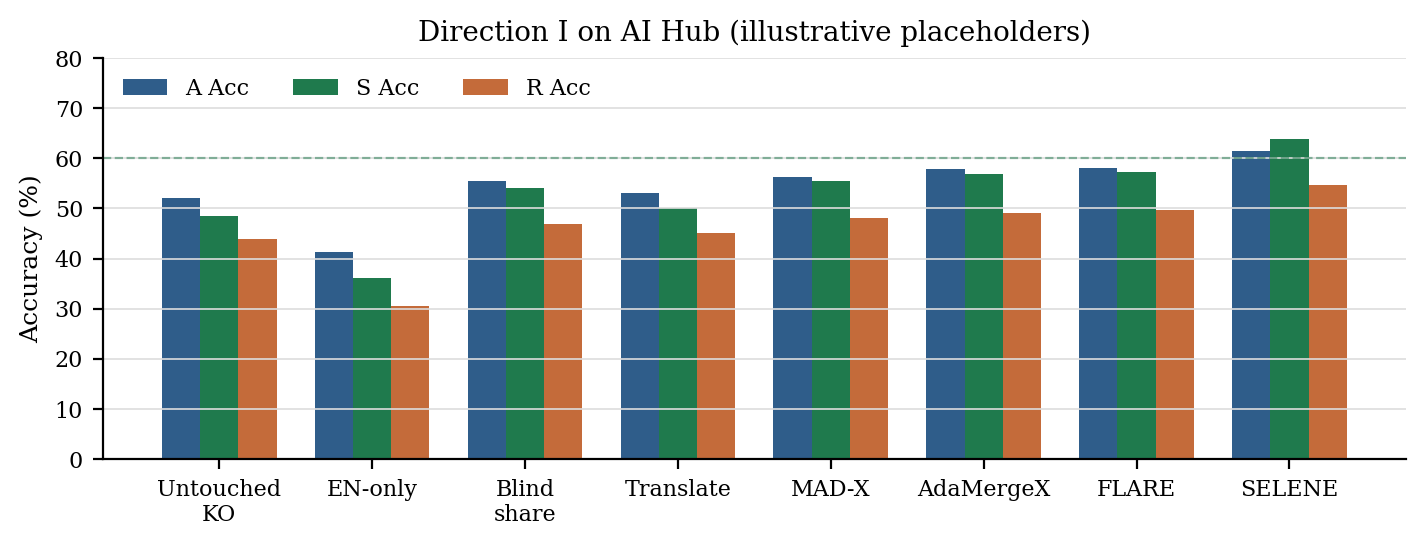
\includegraphics[width=0.92\textwidth]{figures/fig_dir_i_bars.png}
\caption{Direction~I A/S/R Acc on AI~Hub (illustrative placeholders matching Table~\ref{tab:dir_i}).}
\label{fig:dir_i}
\end{figure*}

\subsection{Direction II --- Return to English after KO}
\textbf{Question:} After KO adaptation, is English empathy preserved?
\textbf{Metrics:} ED emotion Acc; $\Delta$Acc / $\Delta$LM vs.\ EN-before-KO.
Table~\ref{tab:dir_ii} and Fig.~\ref{fig:dir_ii} use the same row-as-system style (illustrative placeholders).
KO-scratch induces the largest English drop, while SELENE (and compose $\alpha$) stays near the EN-before reference---echoing less-forgetting multilingual fine-tuning~\cite{wang2022lfmlf,kirkpatrick2017overcoming}.

\begin{table}[!t]
\caption{Direction II: Return-to-EN on EmpatheticDialogues Valid (illustrative placeholders).
$\Delta$ is relative to EN before KO.}
\label{tab:dir_ii}
\centering
\begin{tabular}{@{}lccc@{}}
\toprule
System (adapter on ED) & Acc$\uparrow$ & $\Delta$Acc & $\Delta$LM \\
\midrule
EN before KO & 61.0 & $0.00$ & $0.00$ \\
\midrule
After Untouched KO & 48.2 & $-12.8$ & $+0.37$ \\
After Blind share & 56.5 & $-4.5$ & $+0.05$ \\
After SELENE & 59.8 & $-1.2$ & $+0.01$ \\
After SELENE + $\alpha$ & 60.6 & $-0.4$ & $+0.00$ \\
\bottomrule
\end{tabular}
\end{table}

\begin{figure}[!t]
\centering
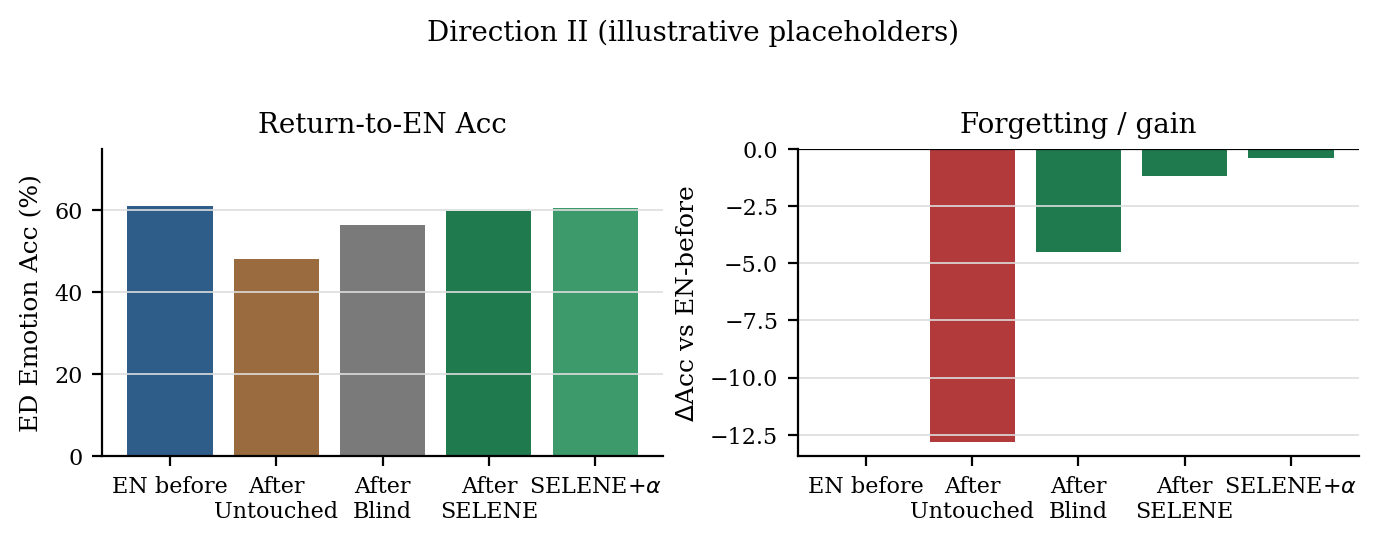
\includegraphics[width=\columnwidth]{figures/fig_dir_ii_bars.png}
\caption{Direction~II return-to-EN Acc and $\Delta$Acc (illustrative placeholders).}
\label{fig:dir_ii}
\end{figure}

\subsection{Stage-Wise Ablation}
Table~\ref{tab:ablation} and Fig.~\ref{fig:ablation} isolate each stage (illustrative placeholders).
Removing Stage~1 (A1) or forcing all-relearn (A5) collapses Dir~I and worsens Dir~II; removing Stage~2 gates (A2) recovers Blind-share behavior; removing A/S/R heads (A3) hurts affective Acc even when LM loss is competitive---confirming multitask heads are not cosmetic~\cite{liu2021esc}.
Fig.~\ref{fig:train} shows Stage~1/3 training curves.

\begin{table}[!t]
\caption{Stage-Wise Ablation (illustrative placeholders).}
\label{tab:ablation}
\centering
\resizebox{\columnwidth}{!}{%
\begin{tabular}{@{}clccc@{}}
\toprule
ID & Configuration & Dir~I Avg$\uparrow$ & Dir~II $\Delta$Acc & Isolates \\
\midrule
A0 & Full SELENE & 60.0 & $-1.2$ & reference \\
A1 & w/o Stage~1 (KO scratch) & 48.2 & $-12.8$ & EN pretrain \\
A2 & w/o Stage~2 (blind share) & 52.1 & $-4.5$ & factor gates \\
A3 & w/o Stage~3 heads (LM only) & 41.0 & $-2.0$ & A/S/R heads \\
A4 & Stage~1 only (no KO train) & 36.0 & $0.0$ & KO adapt \\
A5 & all-relearn & 49.5 & $-11.5$ & share benefit \\
A6 & all-suppress & 50.8 & $-7.0$ & soft unlearn \\
A7 & gate A only & 55.2 & $-2.8$ & single factor \\
A8 & compose $\alpha$ & 59.1 & $-0.4$ & forgetting \\
\bottomrule
\end{tabular}%
}
\end{table}

\begin{figure}[!t]
\centering
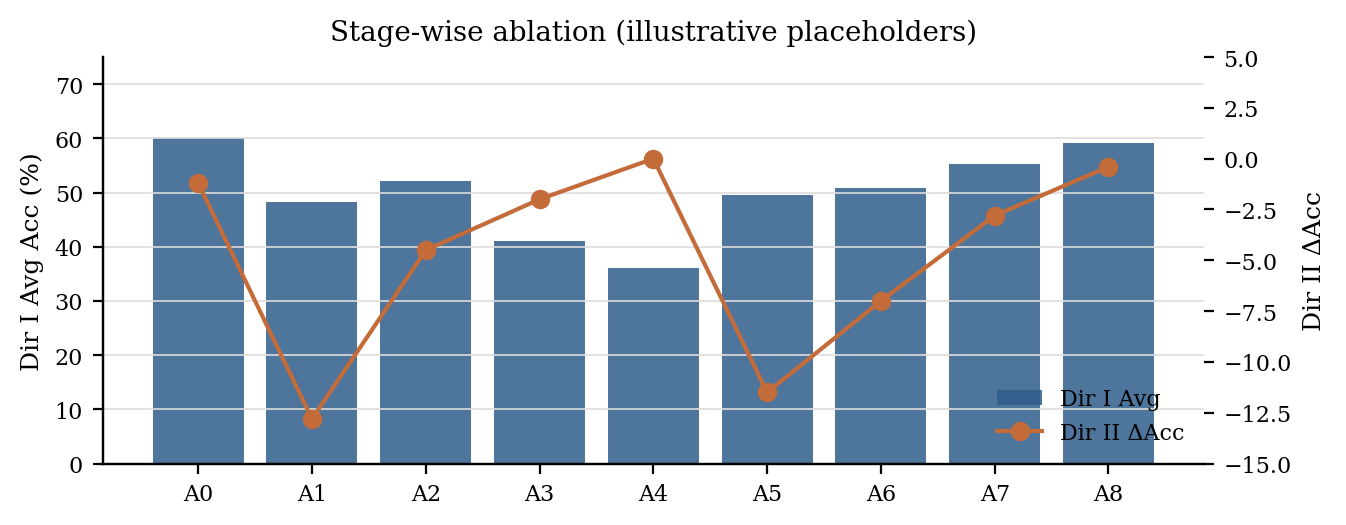
\includegraphics[width=\columnwidth]{figures/fig_ablation.png}
\caption{Stage-wise ablation overview (illustrative placeholders).}
\label{fig:ablation}
\end{figure}

\begin{figure}[!t]
\centering
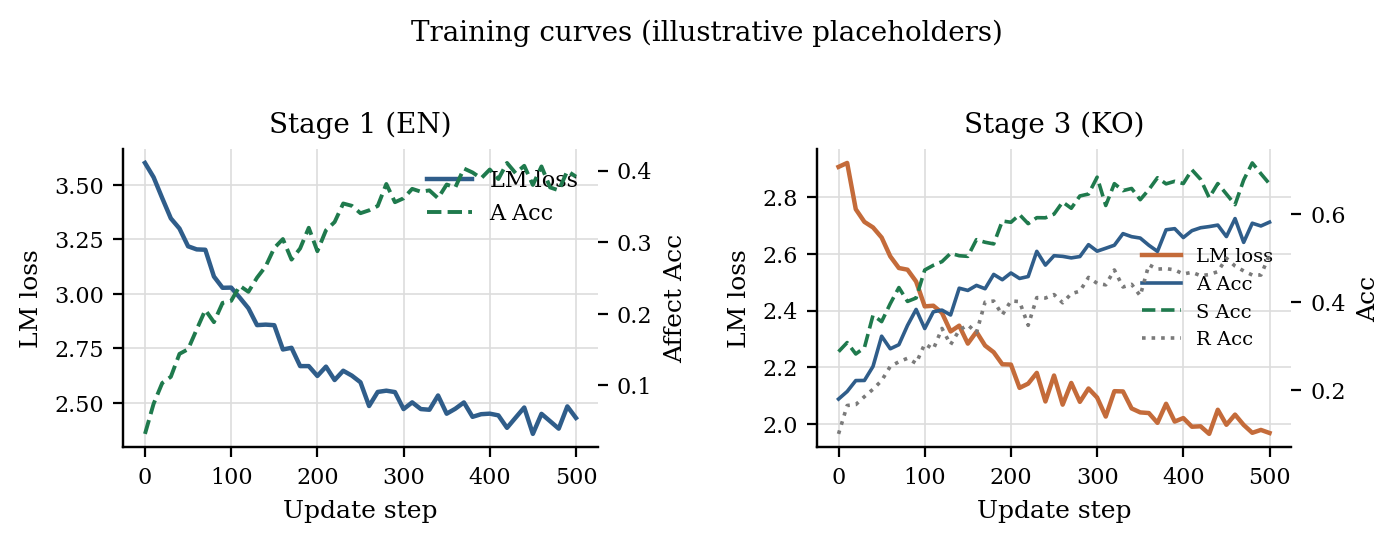
\includegraphics[width=\columnwidth]{figures/fig_train_curves.png}
\caption{Stage~1 (EN) and Stage~3 (KO) training curves (illustrative placeholders).}
\label{fig:train}
\end{figure}

\subsection{Claims}
\begin{itemize}
\item \textbf{Factor pattern:} A/C are EN--KO aligned (share); S/R are KO-specific (relearn)---Fig.~\ref{fig:factor_enko}, Table~\ref{tab:factor_enko}.
\item \textbf{Dir~I:} SELENE $>$ Untouched KO and Blind share on A/S/R (esp.\ S/R), matching ESC's emphasis on strategy~\cite{liu2021esc}.
\item \textbf{Dir~II:} SELENE does not incur larger English forgetting than Blind share; compose $\alpha$ further reduces forgetting~\cite{wang2022lfmlf}.
\item \textbf{Ablation:} removing Stage~2 (A2) or EN pretrain (A1) hurts Dir~I; removing A/S/R heads (A3) hurts affective Acc beyond LM alone.
\end{itemize}

\section{Discussion}
SELENE addresses the cultural empathy gap documented by KoED~\cite{lee2025koed} with a method complementary to language$\times$task XLT~\cite{pfeiffer2020madx,zhao2025adamerge,borchert2025flare}: factor-wise share/relearn/suppress on A/S/R while freezing the backbone.
The EN--KO factor comparison (Fig.~\ref{fig:factor_enko}) is the mechanistic justification for selective gates rather than blind adapter copy: strategy and relation carry Korean interactional norms that English empathy adapters do not encode~\cite{matsumoto2008culture,lee2025koed}, whereas affect and situation appraisal transfer more readily~\cite{davis1983empathy,rashkin2019empathetic}.
This view is consistent with cultural-dominance findings in LLMs~\cite{zhou2024culture} and with multidimensional empathy theory~\cite{davis1983empathy,sharma2020empathy}.
Direction~II follows the less-forgetting intuition of LF-MLF~\cite{wang2022lfmlf} and classical continual-learning warnings~\cite{kirkpatrick2017overcoming}.
Tables~\ref{tab:dir_i}--\ref{tab:ablation} and Figs.~\ref{fig:dir_i}--\ref{fig:train} currently use illustrative placeholders; full Qwen3.5-9B runs will replace them.

\paragraph{Limitations.}
Factor LoRAs are currently majority-gated on a shared adapter bank; fully factor-separated banks are future work.
Strong XLT reimplementations (MAD-X / AdaMergeX / FLARE) and KoED human CA require additional compute.
AI~Hub licensing constrains redistribution of raw dialogues.
Placeholder tables/figures must not be read as submission-ready state-of-the-art rankings.

\section{Conclusion}
We presented \textbf{SELENE}, a selective empathy LoRA system for English--Korean affective transfer on frozen Qwen3.5-9B.
Across factor-wise EN--KO comparisons, Direction~I/II evaluations, and stage ablations, one conclusion emerges:
\textbf{empathy does not transfer as a single skill}---Affect and Cognition are largely shareable from English, whereas Strategy and Relation must be relearned for Korean~\cite{davis1983empathy,liu2021esc,lee2025koed}---so factor-gated adapters improve Korean A/S/R accuracy without the English forgetting induced by KO-scratch or blind overwrite~\cite{wang2022lfmlf}.
Replacing the illustrative placeholders with full Qwen3.5-9B runs and KoED cultural appropriateness scores is the immediate next step.

\section*{Acknowledgments}
The authors thank the maintainers of EmpatheticDialogues, KoED, and AI~Hub for releasing resources that enable culturally grounded empathy research.

\begin{thebibliography}{00}
\bibliographystyle{IEEEtran}

\bibitem{rashkin2019empathetic}
H.~Rashkin, E.~M. Smith, M.~Li, and Y.-L. Boureau, ``Towards empathetic open-domain conversation models: A new benchmark and dataset,'' in \textit{Proc. ACL}, 2019, pp. 5370--5381.

\bibitem{liu2021esc}
S.~Liu \textit{et~al.}, ``Towards emotional support dialog systems,'' in \textit{Proc. ACL}, 2021, pp. 3469--3483.

\bibitem{lee2025koed}
W.~Lee, Y.~Sim, H.~Kim, and H.~Kim, ``Multilingual, not multicultural: Uncovering the cultural empathy gap in LLMs through a comparative empathetic dialogue benchmark,'' in \textit{Proc. IJCNLP-AACL}, 2025, pp. 791--809.

\bibitem{sabour2024emobench}
S.~Sabour \textit{et~al.}, ``EmoBench: Evaluating the emotional intelligence of large language models,'' in \textit{Proc. ACL}, 2024.

\bibitem{hu2022lora}
E.~J.~Hu \textit{et~al.}, ``LoRA: Low-rank adaptation of large language models,'' in \textit{Proc. ICLR}, 2022.

\bibitem{pfeiffer2020madx}
J.~Pfeiffer, I.~Vuli\'{c}, I.~Gurevych, and S.~Ruder, ``MAD-X: An adapter-based framework for multi-task cross-lingual transfer,'' in \textit{Proc. EMNLP}, 2020, pp. 7654--7673.

\bibitem{zhao2025adamerge}
Y.~Zhao \textit{et~al.}, ``AdaMergeX: Cross-lingual transfer with large language models via adaptive adapter merging,'' in \textit{Proc. NAACL}, 2025.

\bibitem{borchert2025flare}
P.~N.~Borchert \textit{et~al.}, ``Language fusion for parameter-efficient cross-lingual transfer,'' in \textit{Proc. ACL}, 2025.

\bibitem{wang2022lfmlf}
Y.~Mao, Y.~Liang, N.~Duan, H.~Wang, K.~Wang, L.~Chen, and Y.~Gao, ``Less-forgetting multi-lingual fine-tuning,'' in \textit{Proc. NeurIPS}, 2022.

\bibitem{davis1983empathy}
M.~H.~Davis, ``Measuring individual differences in empathy: Evidence for a multidimensional approach,'' \textit{J. Pers. Soc. Psychol.}, vol. 44, no. 1, pp. 113--126, 1983.

\bibitem{matsumoto2008culture}
D.~Matsumoto \textit{et~al.}, ``Culture, emotion regulation, and adjustment,'' \textit{J. Pers. Soc. Psychol.}, vol. 94, no. 6, pp. 925--937, 2008.

\bibitem{amin2024chatgpt}
M.~M.~Amin, E.~Cambria, and B.~W.~Schuller, ``A wide evaluation of ChatGPT on affective computing tasks,'' \textit{IEEE Trans. Affect. Comput.}, 2024.


\bibitem{sharma2020empathy}
A.~Sharma, A.~Miner, D.~Atkins, and T.~Althoff, ``A computational approach to understanding empathy expressed in text-based mental health support,'' in \textit{Proc. EMNLP}, 2020, pp. 5263--5276.

\bibitem{lin2019moel}
Z.~Lin \textit{et~al.}, ``MoEL: Mixture of empathetic listeners,'' in \textit{Proc. EMNLP-IJCNLP}, 2019, pp. 133--143.

\bibitem{majumder2020mime}
N.~Majumder \textit{et~al.}, ``MIME: Mimicking emotions for empathetic response generation,'' in \textit{Proc. EMNLP}, 2020, pp. 8968--8979.

\bibitem{sabour2022cem}
S.~Sabour, C.~Zheng, and M.~Huang, ``CEM: Commonsense-aware empathetic response generation,'' in \textit{Proc. AAAI}, 2022, pp. 11229--11237.

\bibitem{zhou2024culture}
W.~Wang \textit{et~al.}, ``Not all countries celebrate Thanksgiving: On the cultural dominance in large language models,'' in \textit{Proc. ACL}, 2024, pp. 6349--6384.

\bibitem{ahuja2023mega}
K.~Ahuja \textit{et~al.}, ``MEGA: Multilingual evaluation of generative AI,'' in \textit{Proc. EMNLP}, 2023, pp. 4232--4267.

\bibitem{ponti2020xcopa}
E.~M.~Ponti \textit{et~al.}, ``XCOPA: A multilingual dataset for causal commonsense reasoning,'' in \textit{Proc. EMNLP}, 2020, pp. 2362--2376.

\bibitem{conneau2020xlmr}
A.~Conneau \textit{et~al.}, ``Unsupervised cross-lingual representation learning at scale,'' in \textit{Proc. ACL}, 2020, pp. 8440--8451.

\bibitem{houlsby2019adapters}
N.~Houlsby \textit{et~al.}, ``Parameter-efficient transfer learning for NLP,'' in \textit{Proc. ICML}, 2019, pp. 2790--2799.

\bibitem{kirkpatrick2017overcoming}
J.~Kirkpatrick \textit{et~al.}, ``Overcoming catastrophic forgetting in neural networks,'' \textit{Proc. Natl. Acad. Sci. U.S.A.}, vol. 114, no. 13, pp. 3521--3526, 2017.


\end{thebibliography}

\begin{IEEEbiographynophoto}{Jaehong Kim}
Jaehong Kim is with the Department of Software Engineering,
Jeonbuk National University, Jeonju, Republic of Korea.
\end{IEEEbiographynophoto}

\begin{IEEEbiographynophoto}{Seohyeon Yoo}
Seohyeon Yoo received the Ph.D. degree and is with the Department of Software Engineering,
Jeonbuk National University, Jeonju, Republic of Korea.
\end{IEEEbiographynophoto}

\begin{IEEEbiographynophoto}{Jaehyuk Cho}
Jaehyuk Cho received the Ph.D. degree and is with the Department of Software Engineering,
Jeonbuk National University, Jeonju, Republic of Korea
(e-mail: chojh@jbnu.ac.kr). He is the corresponding author.
\end{IEEEbiographynophoto}

\end{document}
